\chapter[Acceleration of the Alpha-Eigenvalue Rayleigh Quotient Fixed Point Method by Anderson Acceleration][Anderson Acceleration]{Acceleration of the Alpha-Eigenvalue Rayleigh Quotient Fixed Point Method by Anderson Acceleration}
\label{sec:AndAcc}

Like all fixed-point methods, the alpha-eigenvalue Rayleigh Quotient Fixed Point method exhibits only linear convergence. In most cases, this rate of convergence is acceptable when other methods are unable to converge the alpha-eigenvalue and eigenvector of interest. However, there exists a set of problems where the alpha-eigenvalue Rayleigh Quotient Fixed Point method converges unacceptably slow. These problems are characterized by large domains where neutrons experience a large amount of scattering before finally being absorbed or leaking out of the domain. For these problems, it might become necessary to use acceleration methods to mitigate slow convergence. In this chapter, we discuss the use of \textit{Anderson acceleration} on the Rayleigh Quotient Fixed Point method for alpha-eigenvalue problems. We examine various slow converging criticality problems of interest and describe the performance of Anderson acceleration. We discuss the reduction in transport sweeps, the associated memory costs of the method, and the practical considerations when using Anderson acceleration.

\section{Anderson Acceleration}

We begin by describing Anderson acceleration. Anderson acceleration originated in the work of Anderson \cite{anderson1965iterative} for the solution of nonlinear integral equations. More recently, work by Walker and Ni \cite{walker_anderson_2011} and Toth and Kelley \cite{toth_convergence_2015} have focused on the use of Anderson acceleration in other applications such as multiphysics problems. 

Consider the fixed-point problem
\begin{equation*}
	G(u) = u, \quad G: \mathbb{R}^{N} \rightarrow \mathbb{R}^{N}.
	\label{eq:AAFP}
\end{equation*}
We assume that the iteration converges ($\rho(G'(u^{*})) < 1$) \cite{ostrowski_solution_2016}. Anderson acceleration maintains a history of residuals
\begin{equation}
	f(u) = G(u) - u
\end{equation}
of depth at most $m + 1$, where $m$ is a parameter in the algorithm. An Anderson acceleration iteration that uses $m$ residual histories is referred to as Anderson($m$). Anderson(0) is fixed-point iteration by definition. Anderson acceleration for the fixed-point problem, Eq.~\ref{eq:AAFP}, is given by Algorithm~\ref{algo:AA1}. 
\begin{algorithm}[!htbp]
	\caption{Anderson Acceleration}
	\label{algo:AA1}
	\begin{algorithmic}
		\STATE{Set $u_{0} =$ an initial guess and $m \geq 1$}
		\STATE{$u_{1} = G(u_{0})$}
		\FOR{$n = 0, 1, 2, \cdots$ until convergence}
			\STATE{Set $m_{n} = \min(m,n)$}
			\STATE{Set $F_{n} = (f_{n-m_{n}}, \cdots, f_{n}),$ where $f_{i} = G(u_{i}) - u_{i}$}
			\STATE{Determine $\alpha^{n} = (\alpha_{0}^{(n)}, \cdots, \alpha_{m_{n}}^{(n)})$ that solves $\min_{\alpha} \norm{F_{n} \alpha^{T}}_{2}$ such that $\sum_{i=0}^{m_{n}} \alpha_{i} = 1$}
			\STATE{Set $u_{n+1} = \sum_{i=0}^{m_{n}} \alpha_{i}^{(n)}G(u_{n-m_{n}+i})$}
			\STATE{Test for convergence}
		\ENDFOR
	\end{algorithmic}
\end{algorithm}

Any norm can be used in the minimization step. However, the $\ell_{2}$ is typically used so that the minimization problem can be formulated as a linear least squares problem \cite{walker_anderson_2011}.

In practice, each $m_{n}$ may be further modified to maintain acceptable conditioning of $F_{n}$. In most applications $m_{n}$ is small. $m_{n} = 1$ or $m_{n} = 2$ is common for large systems due to memory constraints and conditioning requirements.

In the original formulation of Anderson acceleration \cite{anderson1965iterative}, the formulation of the next iterate can be made more general using the expression
\begin{align}
	u_{n+1} &= (1-\beta_{n}) \sum_{i=0}^{m_{n}} \alpha_{i}^{(n)} u_{n-m_{n}+i} + \beta_{n} \sum_{i=0}^{m_{n}} \alpha_{i}^{(n)}G(u_{n-m_{n}+i}) \\
	& = \sum_{i=0}^{m_{n}} \alpha_{i}^{(n)} u_{n-m_{n}+i} + \beta_{n} \bigg (  \sum_{i=0}^{m_{n}} \alpha_{i}^{(n)}G(u_{n-m_{n}+i}) - \sum_{i=0}^{m_{n}} \alpha_{i}^{(n)} u_{n-m_{n}+i} \bigg ),
\end{align}
where $\beta_{n}$ is a relaxation parameter. The relaxation parameters $\beta_{n}$ are usually determined heuristically. In practice, $\beta_{n}$ is a damping parameter ($0 < \beta_{n} \leq 1$) and is used to improve convergence by reducing step lengths when iterates are not near the fixed-point solution. Setting $\beta_{n} = 1$ gives the update in Algorithm~\ref{algo:AA1}.

Algorithm~\ref{algo:AA1} requires solving the constrained linear least-squares problem:
\begin{equation}
	min_{\alpha} \norm{F_{n} \alpha^{T}}_{2} \, s.t.\, \sum_{i=0}^{m_{n}} \alpha_{i} = 1.
\end{equation}
Instead, the least squares problem can be formulated \cite{anderson1965iterative} into an equivalent unconstrained problem. This unconstrained Anderson acceleration algorithm is shown in Algorithm~\ref{algo:AA2}.

\clearpage

\begin{algorithm}[!htbp]
	\caption{Unconstrained Anderson Acceleration}
	\label{algo:AA2}
	\begin{algorithmic}
		\STATE{Set $u_{0} =$ an initial guess and $m \geq 1$}
		\STATE{$u_{1} = G(u_{0})$}
		\FOR{$n = 0, 1, 2, \cdots$ until convergence}
			\STATE{Set $m_{n} = \min(m,n)$}
			\STATE{$\Delta F_{n} = (\Delta f_{n-m_{n}}, \cdots, \Delta f_{n-1})$ where $\Delta f_{i} = f_{i+1} - f_{i}$ and $f_{i} = G(u_{i}) - u_{i}$}
			\STATE{Determine $\gamma^{(n)} = (\gamma_{0}^{(n)}, \cdots, \gamma_{m_{n}-1}^{(n)})$ that solves $\min_{\gamma} \norm{f_{n} - \Delta F_{n} \gamma^{T}}_{2}$}
			\STATE{Set $u_{n+1} = G(u_{n}) - \sum_{i=0}^{m_{n}-1} \gamma_{i}^{(n)} \Delta g_{n - m_{n} + i}$ with $\Delta g_{i} = G(u_{i+1}) - G(u_{i})$}
			\STATE{Test for convergence}
		\ENDFOR
	\end{algorithmic}
\end{algorithm}
Determining the coefficients $\gamma^{(n)} = (\gamma_{0}^{(n)}, \cdots, \gamma_{m_{n}-1}^{(n)})$ is done by a QR factorization
\begin{equation}
	\Delta F_{n} = Q_{n}R_{n},
\end{equation}
\begin{equation}
	R_{n} \gamma^{(n)} = Q_{n}^{T}f_{n}.
\end{equation}
The need for a QR factorization increases the computation cost of one iteration of Anderson acceleration. However, various fast and inexpensive QR factorization methods are available. Despite the increased cost per iteration, if Anderson acceleration substantially reduces the number of iterations required for convergence then this cost may be acceptable.

It is usually desirable to do multiple fixed-point iterations before beginning acceleration. Doing fixed-point iterations may allow the vector iterates to get closer to the region of convergence of the fixed point. This is easily implementable in the Anderson acceleration algorithms by prescribing the number of fixed-point iteration evaluations to be done before starting the acceleration.

It is Algorithm~\ref{algo:AA2} that is applied to the acceleration of the alpha-eigenvalue Rayleigh Quotient Fixed Point method.

\section{Anderson Acceleration of Slowly Converging Alpha-Eigenvalue Rayleigh Quotient Fixed Point Problems}

In this section we consider various critical slab problems that are slow to converge using the alpha-eigenvalue Rayleigh Quotient Fixed Point method. These problems are characterized by long slab widths and high amounts of scattering. Since the alpha-eigenvalue is related to the time it takes for a neutron to be absorbed or leak out of the system, the wide slabs with many scattering interactions require many transport sweeps to converge. We apply Anderson acceleration to these problems and explore the performance of the acceleration method for various parameters of the method. We look at the effects of the number of residual vectors used in the calculation of the next iterate, the number of initial fixed-point iterations done before beginning acceleration, and the impacts of the relaxation parameter $\beta_{n}$. All calculations were done in Matlab \cite{MATLAB:2019}, with reference eigenvalues determined by forming the neutron transport matrices and the Matlab eigenvalue function to determine the dominant alpha-eigenvalue. The implementation of Anderson acceleration used to examine these problems is shown in Appendix~\ref{AnderAccMATLAB}.

\subsection{Uranium-Heavy Water Critical Slab (Sood Criticality Benchmark Problem 68)}

In Section~\ref{sec:MGMultSlabs}, the uranium-heavy water critical slab problem, Sood Criticality Problem 68, was examined. The problem was characterized by large in-group scattering cross sections and a large critical width. Due to these characteristics, the Rayleigh Quotient Fixed Point method for alpha-eigenvalue problems was slow to converge. Unlike previous problems, Sood Criticality Problem 68 required hundreds of thousands of transport sweeps to converge. We reexamine Sood Criticality Problem 68 and apply Anderson acceleration. The problem cross sections are seen in Chapter 6, Table~\ref{table:D2O} and the problem critical width and reference alpha-eigenvalue for one hundred spatial cells, step-differencing, and S$_{16}$ discrete ordinates angular quadrature are shown in Table~\ref{table:Sood68Ref}.

\begin{table}[b]
\caption{Sood Criticality Problem 68 Critical Width and Reference Alpha-Eigenvalue \cite{sood2003analytical}}
	\label{table:Sood68Ref}
	\begin{subtable}[h]{1.0\textwidth}
	\centering\ra{1.3}
	\begin{tabular}{@{}ccc@{}}\toprule
	Cross Section Set & r$_{c}$ [cm] & Reference $\alpha$ [s$^{-1}$] \\
	\midrule
	U-D$_{2}$O(68) & 846.632726 & $-1.508539 \times 10^{-5}$ \\
	\bottomrule%
	\multicolumn{3}{l}{$M = 100$, $L = 16$, Tolerance = $10^{-12}$} \\
	\end{tabular}
	\end{subtable}%
\end{table}

The number of iterations required to converge the eigenvalue/eigenvector fixed point is shown in Table~\ref{table:Sood68AA}. In this chapter, we define one iteration to equal the transport sweep plus the cost of the Anderson acceleration. It follows that for the alpha-eigenvalue Rayleigh Quotient Fixed Point Method, one iteration is equal to one transport sweep. Zero, five, ten, 20, 50, and 100 fixed point iterations were done before beginning acceleration. Table~\ref{table:Sood68AA} shows results for relaxation parameter $\beta_{n} = 1$. The Rayleigh Quotient Fixed Point method (Anderson(0)) required 23796 transport sweeps to converge to the fixed point to a $\ell_{2}$ residual tolerance of $10^{-8}$. The tolerance for Anderson accelerated calculations was set to $10^{-12}$ to prevent false convergence as mentioned in \cite{walker_anderson_2011}. For zero initial fixed-point iterations, it is seen that Anderson(1), the variant of the method which only keeps the most current residual vector, does not converge to the correct eigenvalue. Increasing the number of residual vectors allows the method to converge to the correct eigenvalue and results in substantial reductions in the number of iterations required for convergence. Each additional residual vector is of size $GLM$ and using many residual vectors quickly becomes untenable for large problems. 

Figure~\ref{fig:AASoodProb68} shows the convergence behavior of the Anderson acceleration variants that converge to the correct eigenvalue. Compared to the monotonic decrease in the residual of the Rayleigh Quotient Fixed Point method, the Anderson acceleration variants show significant oscillations. These oscillations make it possible to converge prematurely and for this reason a tighter tolerance is required. The increase of residual vectors used damped out the oscillations faster and allowed the acceleration method to converge with fewer iterations at the cost of additional memory.

Given the tendency of the acceleration method to oscillate, the relaxation parameter $\beta_{n}$ can be used to reduce these oscillations. For relaxation parameter $\beta_{n} = 0.5$, Figure~\ref{fig:AASoodProb68HalfBeta} shows the convergence of behavior of Anderson acceleration. The relaxation parameter increased the number of iterations required to converge the problem but also allowed for the Anderson(1) variant of the problem to converge to the correct eigenvalue though it underperformed Anderson(0) acceleration. This increase in iterations is seen in the shift of the residual to the right in Figure~\ref{fig:AASoodProb68HalfBeta}. The relaxation parameter $\beta_{n}$ can be used to force the method to converge to the correct fixed point at the cost of additional iterations.

For an increasing number of initial fixed-point iterations, we see in Table~\ref{table:Sood68AA} that this resulted in the reduction of iterations required to converge to the fixed point. The preliminary fixed-point iterations allowed for the iterates to approach the region of convergence of the fixed point. The additional fixed-point iterations allow other Anderson acceleration variants to converge to the correct eigenvalue/eigenvector that would otherwise not converge to the the correct fixed point.

In most variants of Anderson acceleration, we see that increasing the number of residual vectors improves the performance of the acceleration method. However, in certain circumstances we see that using five vectors degraded the performance of the method. In these cases, it is thought that the condition number of the system has become large. This can be avoid by deleting rows of the system. However, given this fact, for Sood Criticality Benchmark Problem 68, it is recommended that three or four residual vectors be used with any number of initial fixed-point iterations or relaxation parameter $\beta_{n}$. Anderson acceleration provides substantial reductions in the number of iterations required for converge despite it requiring a tighter tolerance and being more expensive than the alpha-eigenvalue Rayleigh Quotient Fixed Point method.

\begin{table}[!htbp]
\caption{Anderson Acceleration for Sood Criticality Problem 68 ($\beta_{n} = 1, M = 100, L = 16$)}
	\label{table:Sood68AA}
	\begin{subtable}[h]{1.0\textwidth}
	\centering\ra{1.3}
	\begin{tabular}{@{}ccc@{}}\toprule
	Anderson($m_{n}$) & Calculated $\alpha$ [s$^{-1}$] & Iterations \\
	\midrule
	Anderson(0) & $-1.508539 \times 10^{-5}$ & 23796 \\
	Anderson(1) & $-8.790638 \times 10^{-4}$ & 30872 \\
	Anderson(2) & $-1.508539 \times 10^{-5}$ & 7130 \\
	Anderson(3) & $-1.508539 \times 10^{-5}$ & 6976 \\
	Anderson(4) & $-1.508539 \times 10^{-5}$ & 3596 \\
	Anderson(5) & $-1.508539 \times 10^{-5}$ & 2668 \\
	\bottomrule
	Initial Fixed-Point Iterations = 0
	\end{tabular}
	\end{subtable}%
	\vspace{0.25cm}
	\begin{subtable}[h]{1.0\textwidth}
	\centering\ra{1.3}
	\begin{tabular}{@{}ccc@{}}\toprule
	Anderson($m_{n}$) & Calculated $\alpha$ [s$^{-1}$] & Iterations \\
	\midrule
	Anderson(1) & $-8.790638 \times 10^{-4}$ & 19447 \\
	Anderson(2) & $-1.508539 \times 10^{-5}$ & 8782 \\
	Anderson(3) & $-1.508539 \times 10^{-5}$ & 3148 \\
	Anderson(4) & $-1.508539 \times 10^{-5}$ & 1964 \\
	Anderson(5) & $-1.508539 \times 10^{-5}$ & 2624 \\
	\bottomrule
	Initial Fixed-Point Iterations = 5
	\end{tabular}
	\end{subtable}%
	\vspace{0.25cm}
	\begin{subtable}[h]{1.0\textwidth}
	\centering\ra{1.3}
	\begin{tabular}{@{}ccc@{}}\toprule
	Anderson($m_{n}$) & Calculated $\alpha$ [s$^{-1}$] & Iterations \\
	\midrule
	Anderson(1) & $-1.508539 \times 10^{-5}$ & 18514 \\
	Anderson(2) & $-1.508539 \times 10^{-5}$ & 5813 \\
	Anderson(3) & $-1.508539 \times 10^{-5}$ & 4664 \\
	Anderson(4) & $-1.508539 \times 10^{-5}$ & 2806 \\
	Anderson(5) & $-1.508539 \times 10^{-5}$ & 4669 \\
	\bottomrule
	Initial Fixed-Point Iterations = 10
	\end{tabular}
	\end{subtable}
\end{table}

\begin{table}[!htbp]\ContinuedFloat
	\begin{subtable}[h]{1.0\textwidth}
	\centering\ra{1.3}
	\begin{tabular}{@{}ccc@{}}\toprule
	Anderson($m_{n}$) & Calculated $\alpha$ [s$^{-1}$] & Iterations \\
	\midrule
	Anderson(1) & $-1.508539 \times 10^{-5}$ & 16665 \\
	Anderson(2) & $-1.508539 \times 10^{-5}$ & 5944 \\
	Anderson(3) & $-1.508539 \times 10^{-5}$ & 5430 \\
	Anderson(4) & $-1.508539 \times 10^{-5}$ & 1498 \\
	Anderson(5) & $-1.508539 \times 10^{-5}$ & 1729 \\
	\bottomrule
	Initial Fixed-Point Iterations = 20
	\end{tabular}
	\end{subtable}%
	\vspace{0.25cm}
	\begin{subtable}[h]{1.0\textwidth}
	\centering\ra{1.3}
	\begin{tabular}{@{}ccc@{}}\toprule
	Anderson($m_{n}$) & Calculated $\alpha$ [s$^{-1}$] & Iterations \\
	\midrule
	Anderson(1) & $-1.508539 \times 10^{-5}$ & 13396 \\
	Anderson(2) & $-1.508539 \times 10^{-5}$ & 10641 \\
	Anderson(3) & $-1.599327 \times 10^{-4}$ & 8375 \\
	Anderson(4) & $-1.508539 \times 10^{-5}$ & 3441 \\
	Anderson(5) & $-1.508539 \times 10^{-5}$ & 2416 \\
	\bottomrule
	Initial Fixed-Point Iterations = 50
	\end{tabular}
	\end{subtable}%
	\vspace{0.25cm}
	\begin{subtable}[h]{1.0\textwidth}
	\centering\ra{1.3}
	\begin{tabular}{@{}ccc@{}}\toprule
	Anderson($m_{n}$) & Calculated $\alpha$ [s$^{-1}$] & Iterations \\
	\midrule
	Anderson(1) & $-1.508539 \times 10^{-5}$ & 11729 \\
	Anderson(2) & $-1.508539 \times 10^{-5}$ & 7066 \\
	Anderson(3) & $-1.508539 \times 10^{-5}$ & 4748 \\
	Anderson(4) & $-1.508539 \times 10^{-5}$ & 1894 \\
	Anderson(5) & $-1.508539 \times 10^{-5}$ & 3280 \\
	\bottomrule
	Initial Fixed-Point Iterations = 100
	\end{tabular}
	\end{subtable}
\end{table}

\begin{figure}[!htbp]
\centering
\begin{subfigure}{\textwidth}
  \centering
  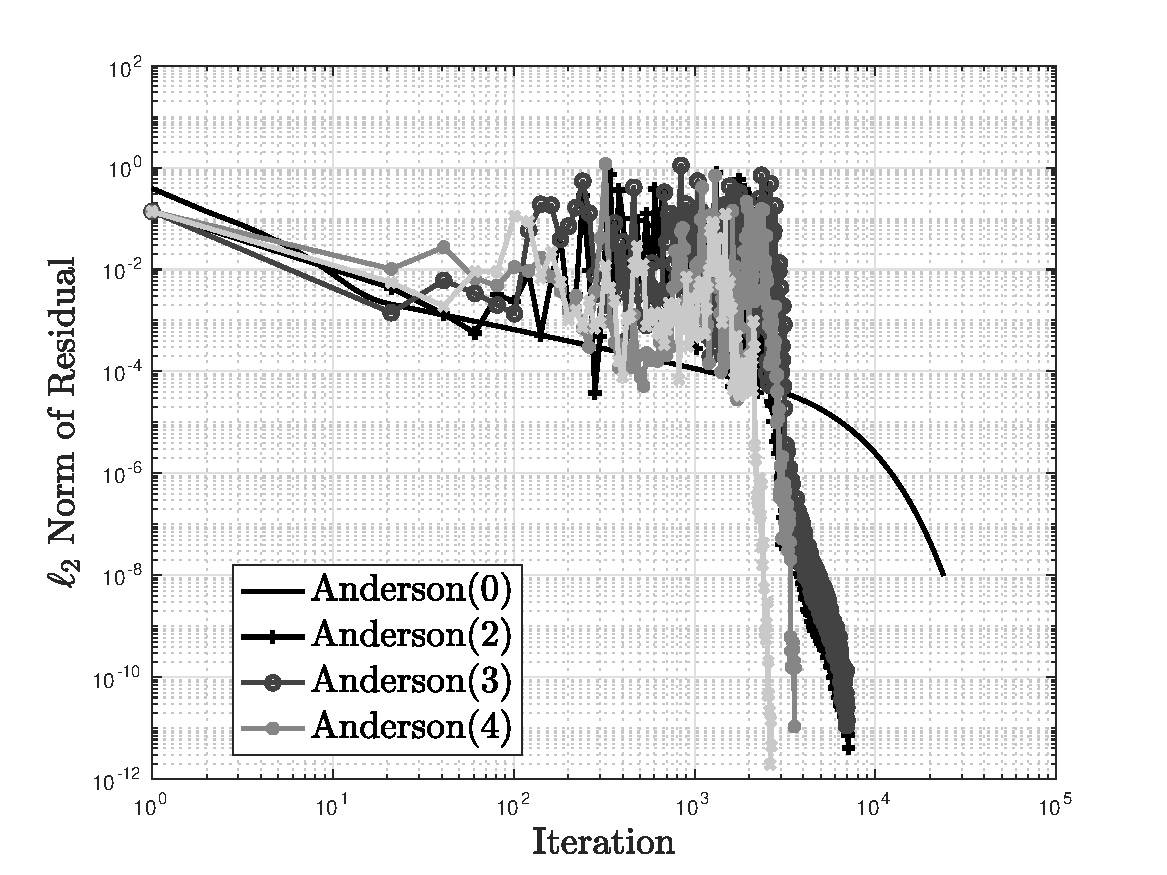
\includegraphics[width=.75\linewidth]{Figures/AndersonAcceleration/SoodProb68_FPI1}
\end{subfigure}
\caption{Anderson Acceleration Convergence for Sood Criticality Problem 68 ($\beta_{n} = 1$)}
\label{fig:AASoodProb68}
\end{figure}

\begin{figure}[!htbp]
\centering
\begin{subfigure}{\textwidth}
  \centering
  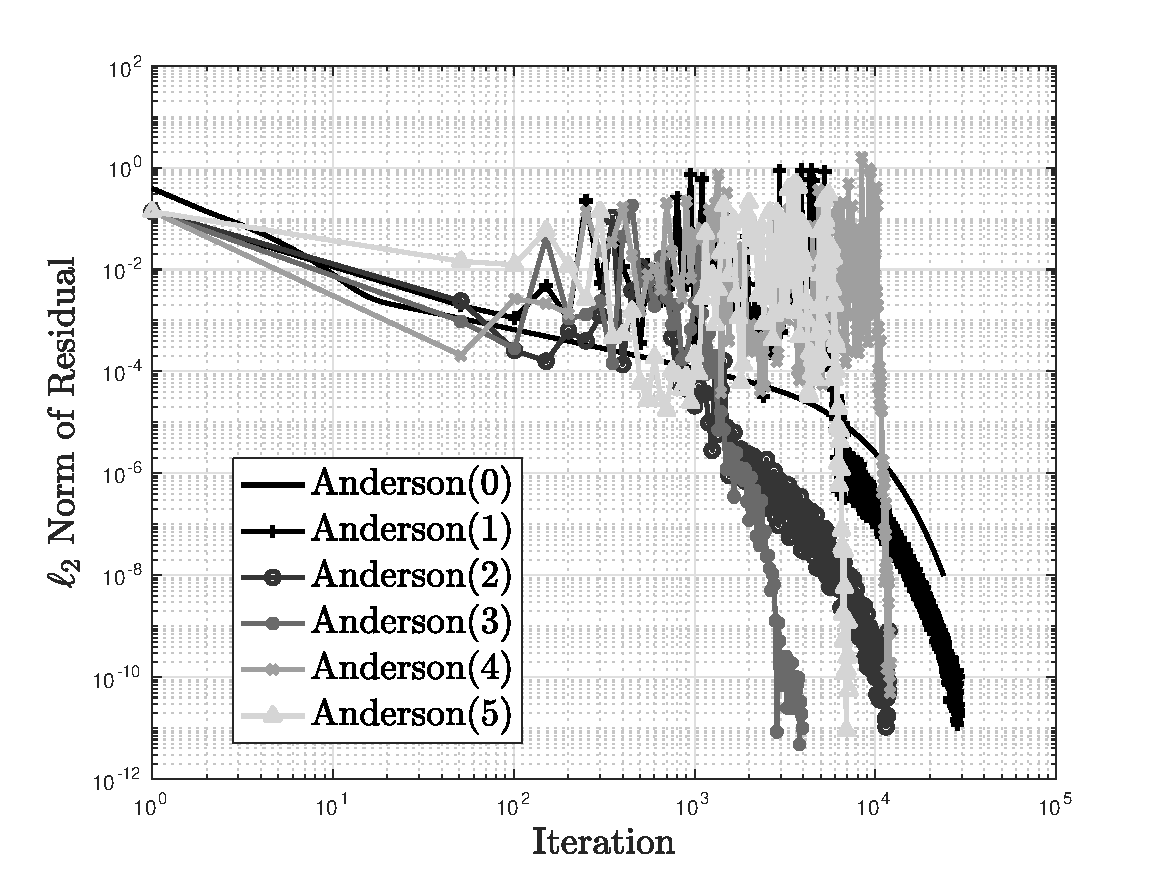
\includegraphics[width=.75\linewidth]{Figures/AndersonAcceleration/SoodProb68_FPI1_HalfBeta}
\end{subfigure}
\caption{Anderson Acceleration Convergence for Sood Criticality Problem 68 ($\beta_{n} = 0.5$)}
\label{fig:AASoodProb68HalfBeta}
\end{figure}

\clearpage

\subsection{Uranium-Heavy Water Critical Slab (Sood Criticality Benchmark Problem 73)}

In this section we examine another uranium-heavy water critical slab problem that is slow to converge when using the Rayleigh Quotient Fixed Point method. Similar to Sood Criticality Benchmark Problem 68, Sood Criticality Benchmark Problem 73 has large amounts of scattering and a large critical width. This problem also contains anisotropic scattering where some of these cross sections are negative. Table~\ref{table:D2O-Sood73} lists the two-group cross sections and Table~\ref{table:Sood73Ref} lists the critical width of the slab and the reference alpha-eigenvalue. The problem was modeled using one hundred spatial cells, step differencing, and S$_{16}$ discrete ordinates angular quadrature.

The number of iterations required to converge the eigenvalue/eigenvector is shown in Table~\ref{table:Sood73AA}. Zero, five, ten, 20, 50, and 100 preliminary fixed-point iteration variants were studied with relaxation factor $\beta_{n} = 1$. The Rayleigh Quotient Fixed Point (Anderson(0)) required 22749 iterations to converge the eigenvalue/eigenvector to an $\ell_{2}$ residual of $10^{-8}$. As before, the tolerance of the Anderson acceleration calculations was set to $10^{-12}$ to prevent false convergence. Unlike Sood Criticality Benchmark Problem 68, it was found that all Anderson acceleration variants converged to the correct eigenvalue. As the number of residual vectors increased, the number of iterations decreased except in the case of five residual vectors. For this number of residual vectors, it was found that the linear system was poorly conditioned.

Figure~\ref{fig:AASoodProb73} shows the convergence behavior of the different Anderson acceleration variants ($\beta_{n} = 1$, zero initial fixed-point iterations) and the Rayleigh Quotient Fixed Point method. The Anderson acceleration variants oscillate substantially until converging to the fixed point. While Anderson(1) only reduced the number of iterations required by a factor of 20\%, Anderson(3) and Anderson(4) reduced iteration number by up to factor of 10. Using relaxation parameter $\beta_{n} = 0.5$, the number of iterations increased. We see a shift toward the right of the convergence behavior in Figure~\ref{fig:AASoodProb73Half}. For this particular problem, the relaxation parameter is not necessary since all Anderson acceleration variants converge onto the right fixed point.

Increasing the number of initial fixed-point iterations before acceleration only reduces the number of total iterations in some cases. As the number of initial fixed-point iterations increases, it was seen that the number of iterations either remained the same or increased (Table~\ref{table:Sood73AA}). By allowing for more initial iterations, it is possible that the vector iterates ended up much further from the fixed point. If instead the acceleration were turned on sooner, the iterates would instead end up in the region of convergence much sooner.

For this particular problem, Anderson acceleration provided substantial reductions in iterations. However, for certain combinations of residual vector number, relaxation parameters, and initial fixed-point iterations, it was found that the acceleration method would not perform as well. Similar to the previous problem, using three or four residual vectors with five or ten initial fixed-point iterations was found to give the best results. This problem, however, shows that the various parameters of Anderson acceleration require experimentation in order to find the best results.

\begin{table}[!htbp]
	\caption{Two-Group U-D$_{2}$O Problem Cross Sections (cm$^{-1}$)}
	\label{table:D2O-Sood73}
	\begin{subtable}[!htbp]{1.0\textwidth}
		\centering\ra{1.3}
		\begin{tabular}{@{}cccccc@{}}\toprule
			$g$ & $\sigma_{g} $ & $\nu_{g}$ & $\sigma_{fg}$ & $\chi_{g}$ & $v_{g}$ [cm/s] \\ 
        			\midrule
			1 & 0.33588  & 2.50 & 0.002817 & 1.0 & 2.0 \\
			2 & 0.54628  & 2.50 & 0.097 & 0.0 & 1.0 \\
			\bottomrule
		\end{tabular}
	\caption{U-D$_{2}$O(73) Cross Sections}
	\end{subtable}%
	\vspace{0.25cm}
	\begin{subtable}[!htbp]{1.0\textwidth}
	\centering\ra{1.3}
	\begin{tabular}{@{}ccc@{}}\toprule
	$g' \rightarrow g$ & 1 & 2 \\ 
        \midrule
	1 & 0.31980 & 0.004555   \\
	2 & 0.0 & 0.42410  \\
	\bottomrule
	\end{tabular}
	\caption{U-D$_{2}$O(73) Scattering Block-$\sigma_{s0}$}
	\end{subtable}
		\begin{subtable}[!htbp]{1.0\textwidth}
	\centering\ra{1.3}
	\begin{tabular}{@{}ccc@{}}\toprule
	$g' \rightarrow g$ & 1 & 2 \\ 
        \midrule
	1 & 0.06694 & -0.0003972 \\
	2 & 0.0 & 0.05439  \\
	\bottomrule
	\end{tabular}
	\caption{U-D$_{2}$O(73) Scattering Block-$\sigma_{s1}$}
	\end{subtable}
\end{table}

\begin{table}[!htbp]
\caption{Sood Criticality Problem 73 Critical Width and Reference Alpha-Eigenvalue \cite{sood2003analytical}}
	\label{table:Sood73Ref}
	\begin{subtable}[h]{1.0\textwidth}
	\centering\ra{1.3}
	\begin{tabular}{@{}ccc@{}}\toprule
	Cross Section Set & r$_{c}$ [cm] & Reference $\alpha$ [s$^{-1}$] \\
	\midrule
	U-D$_{2}$O(73) & 1000.506133 & $-1.221913 \times 10^{-5}$ \\
	\bottomrule
	\multicolumn{3}{l}{$M = 100$, $L = 16$, Tolerance = $10^{-12}$} \\
	\end{tabular}
	\end{subtable}%
\end{table}

\begin{table}[!htbp]
\caption{Anderson Acceleration for Sood Criticality Problem 73 ($\beta_{n} = 1, M = 100, L = 16$)}
	\label{table:Sood73AA}
	\begin{subtable}[h]{1.0\textwidth}
	\centering\ra{1.3}
	\begin{tabular}{@{}ccc@{}}\toprule
	Anderson($m_{n}$) & Calculated $\alpha$ [s$^{-1}$] & Iterations \\
	\midrule
	Anderson(0) & $-1.221913 \times 10^{-5}$ & 22749 \\
	Anderson(1) & $-1.221913 \times 10^{-5}$ & 17620 \\
	Anderson(2) & $-1.221913 \times 10^{-5}$ & 4814  \\
	Anderson(3) & $-1.221913 \times 10^{-5}$ & 2777  \\
	Anderson(4) & $-1.221913 \times 10^{-5}$ & 1854  \\
	Anderson(5) & $-1.221913 \times 10^{-5}$ & 6008  \\
	\bottomrule
	Initial Fixed-Point Iterations = 0
	\end{tabular}
	\end{subtable}%
	\vspace{0.25cm}
	\begin{subtable}[h]{1.0\textwidth}
	\centering\ra{1.3}
	\begin{tabular}{@{}ccc@{}}\toprule
	Anderson($m_{n}$) & Calculated $\alpha$ [s$^{-1}$] & Iterations \\
	\midrule
	Anderson(1) & $-1.221913 \times 10^{-5}$ & 17775 \\
	Anderson(2) & $-1.221913 \times 10^{-5}$ & 9204 \\
	Anderson(3) & $-1.221913 \times 10^{-5}$ & 2583 \\
	Anderson(4) & $-1.221913 \times 10^{-5}$ & 1407 \\
	Anderson(5) & $-1.221913 \times 10^{-5}$ & 6172 \\
	\bottomrule
	Initial Fixed-Point Iterations = 5
	\end{tabular}
	\end{subtable}%
	\vspace{0.25cm}
	\begin{subtable}[h]{1.0\textwidth}
	\centering\ra{1.3}
	\begin{tabular}{@{}ccc@{}}\toprule
	Anderson($m_{n}$) & Calculated $\alpha$ [s$^{-1}$] & Iterations \\
	\midrule
	Anderson(1) & $-1.221913 \times 10^{-5}$ & 12186 \\
	Anderson(2) & $-1.221913 \times 10^{-5}$ & 11382 \\
	Anderson(3) & $-1.221913 \times 10^{-5}$ & 4809 \\
	Anderson(4) & $-1.221913 \times 10^{-5}$ & 2626 \\
	Anderson(5) & $-1.221913 \times 10^{-5}$ & 3603 \\
	\bottomrule
	Initial Fixed-Point Iterations = 10
	\end{tabular}
	\end{subtable}
\end{table}

\begin{table}[!htbp]\ContinuedFloat
	\begin{subtable}[h]{1.0\textwidth}
	\centering\ra{1.3}
	\begin{tabular}{@{}ccc@{}}\toprule
	Anderson($m_{n}$) & Calculated $\alpha$ [s$^{-1}$] & Iterations \\
	\midrule
	Anderson(1) & $-1.221913 \times 10^{-5}$ & 12241 \\
	Anderson(2) & $-1.221913 \times 10^{-5}$ & 3604  \\
	Anderson(3) & $-1.221913 \times 10^{-5}$ & 6713  \\
	Anderson(4) & $-1.221913 \times 10^{-5}$ & 5430  \\
	Anderson(5) & $-1.221913 \times 10^{-5}$ & 2925  \\
	\bottomrule
	Initial Fixed-Point Iterations = 20
	\end{tabular}
	\end{subtable}%
	\vspace{0.25cm}
	\begin{subtable}[h]{1.0\textwidth}
	\centering\ra{1.3}
	\begin{tabular}{@{}ccc@{}}\toprule
	Anderson($m_{n}$) & Calculated $\alpha$ [s$^{-1}$] & Iterations \\
	\midrule
	Anderson(1) & $-1.221913 \times 10^{-5}$ & 17166 \\
	Anderson(2) & $-1.221913 \times 10^{-5}$ & 7363 \\
	Anderson(3) & $-1.221913 \times 10^{-5}$ & 4205 \\
	Anderson(4) & $-1.221913 \times 10^{-5}$ & 1729 \\
	Anderson(5) & $-1.221913 \times 10^{-5}$ & 2253 \\
	\bottomrule
	Initial Fixed-Point Iterations = 50
	\end{tabular}
	\end{subtable}%
	\vspace{0.25cm}
	\begin{subtable}[h]{1.0\textwidth}
	\centering\ra{1.3}
	\begin{tabular}{@{}ccc@{}}\toprule
	Anderson($m_{n}$) & Calculated $\alpha$ [s$^{-1}$] & Iterations \\
	\midrule
	Anderson(1) & $-1.221913 \times 10^{-5}$ & 17313 \\
	Anderson(2) & $-1.221913 \times 10^{-5}$ & 14811 \\
	Anderson(3) & $-1.221913 \times 10^{-5}$ & 10654 \\
	Anderson(4) & $-1.221913 \times 10^{-5}$ & 3923 \\
	Anderson(5) & $-1.221913 \times 10^{-5}$ & 3657 \\
	\bottomrule
	Initial Fixed-Point Iterations = 100
	\end{tabular}
	\end{subtable}
\end{table}

\begin{figure}[!htbp]
\centering
\begin{subfigure}{\textwidth}
  \centering
  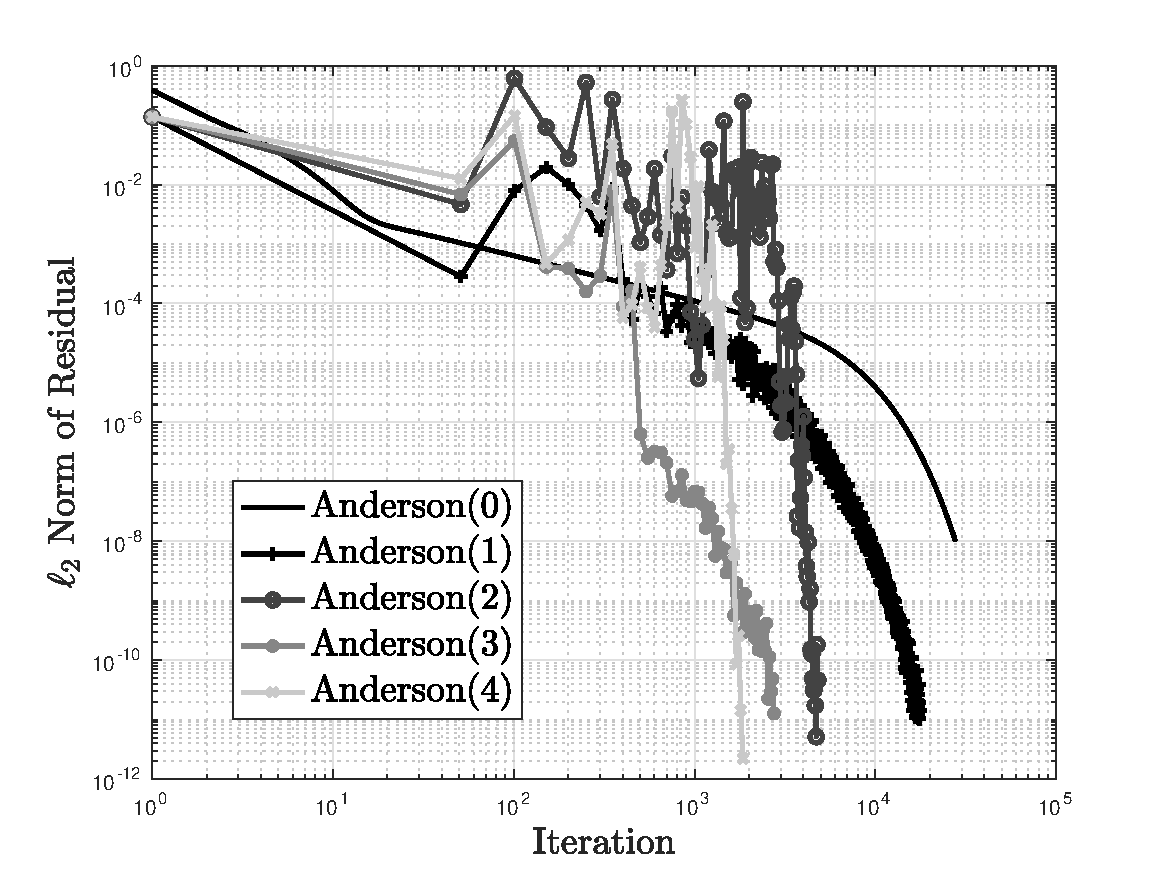
\includegraphics[width=.75\linewidth]{Figures/AndersonAcceleration/SoodProb73}
\end{subfigure}
\caption{Anderson Acceleration Convergence for Sood Criticality Problem 73 ($\beta_{n} = 1$)}
\label{fig:AASoodProb73}
\end{figure}

\begin{figure}[!htbp]
\centering
\begin{subfigure}{\textwidth}
  \centering
  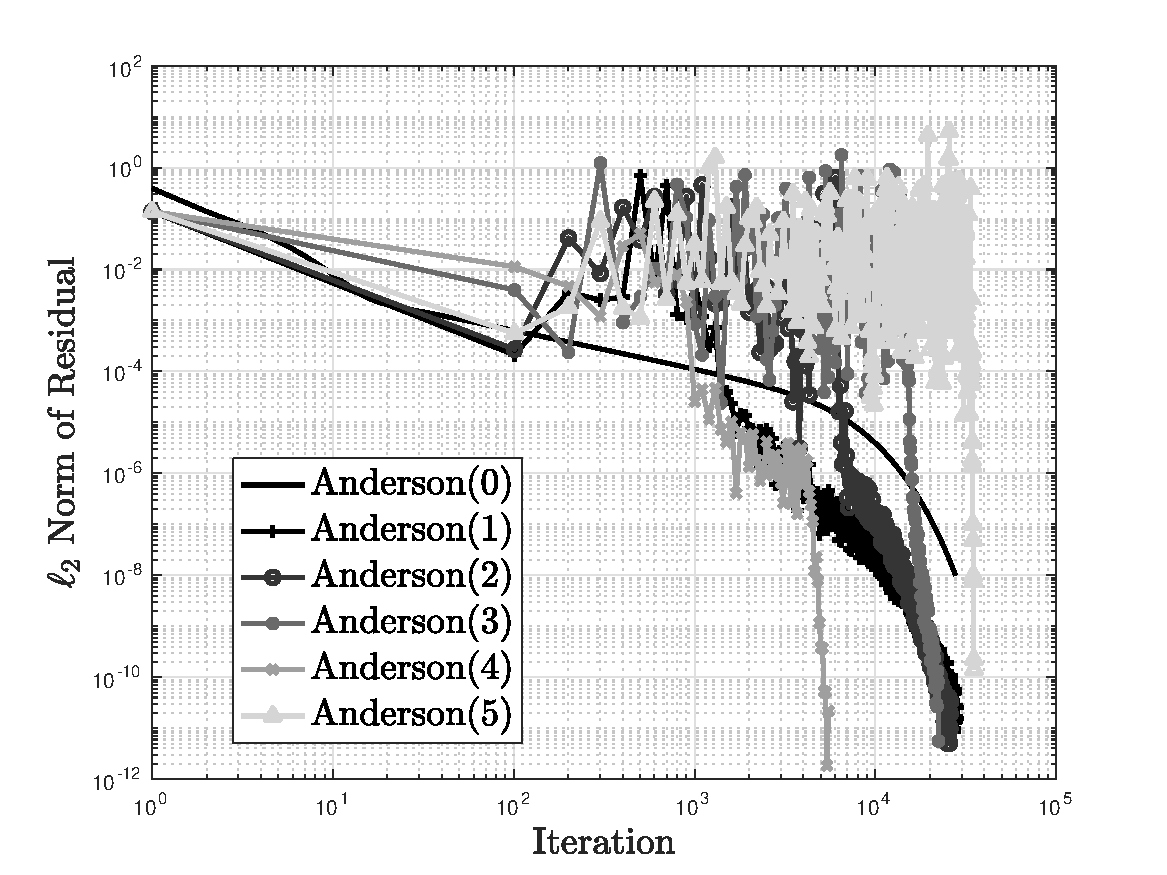
\includegraphics[width=.75\linewidth]{Figures/AndersonAcceleration/SoodProb73_FPI1_HalfBeta}
\end{subfigure}
\caption{Anderson Acceleration Convergence for Sood Criticality Problem 73 ($\beta_{n} = 0.5$)}
\label{fig:AASoodProb73Half}
\end{figure}

\clearpage

\section{Conclusion}

Anderson acceleration was applied to the Rayleigh Quotient Fixed Point method for alpha-eigenvalue problems. Anderson acceleration and its constrained and unconstrained formulations were presented. The unconstrained formulation of Anderson acceleration was implemented in MATLAB and applied to the RQFP method. Two slowly converging one-dimensional slab geometry problems were considered and the number of iterations compared for various variants of the acceleration scheme. The effects of different numbers of residual vectors and initial fixed-point iterations before acceleration were considered and their effects on the ability of the method to converge to the fundamental eigenvector and eigenvalue were discussed. It was found that while larger numbers of residual vectors produced faster convergence, memory limitations quickly became apparently. Instead it was found that by using a combination of initial fixed-point iterations and a lesser number of residual vectors produced substantial speedups. In particular, the initial fixed-point iterations were found to help the method to converge to the correct eigenpair by allowing the vector iterate to enter the region of convergence for the fixed point.